\documentclass[submit,noauthor]{ono}
% \documentclass[submit,techrep,noauthor]{ipsj}
%\documentclass{ipsj}
\usepackage[dvipdfmx]{graphicx}
\usepackage{graphicx}
\usepackage{float}
\usepackage{url}
\usepackage{lmodern}
\usepackage{booktabs}
\usepackage{tabularx} 

\def\Underline{\setbox0\hbox\bgroup\let\\\endUnderline}
\def\endUnderline{\vphantom{y}\egroup\smash{\underline{\box0}}\\}
\def\|{\verb|}

% \setcounter{巻数}{59}
% \setcounter{号数}{1}
% \setcounter{page}{1}

\受付{2016}{3}{4}
\採録{2016}{8}{1}

\begin{document}

\title{論文タイトル\\}

\etitle{English Title ssample \\
	(kakkokako)}

\paffiliate{JU}{東京大学駒場図書館\\
	Komaba Library, University of Tokyo}

\author{小野 亘}{Wataru, ONO}{utokyo}[ono.wataru@mail.u-tokyo.ac.jp]

\begin{abstract}
	本稿は,NII 等をまとめたものであるよね.
\end{abstract}


\begin{jkeyword}
	情報処理学会論文誌ジャーナル,\LaTeX,スタイルファイル,べからず集
\end{jkeyword}

\begin{eabstract}
	This document is
\end{eabstract}

\begin{ekeyword}
	IPSJ Journal, \LaTeX, style files, ``Dos and Don'ts'' list
\end{ekeyword}

\maketitle

%1
\section{はじめに}

本稿では,国立情報学(NII)のIRDBから統計データを取得し、
日本の機関リポジトリに登録されたコンテンツの種別(資源タイプ)の分析を行い、
その側面から、日本の機関リポジトリの特徴を明らかにするものである。

\footnotetext{https://irdb.nii.ac.jp/}

%2
\section{方法}
今回は、Python 3.10.7、Pandas 1.5.2 を使用した。

%3
\section{結論}

%4
\section{データの読み込み、前処理}
%4.1
\subsection{準備}

NIIのIRDBの「コンテンツ統計(全体)」から、統計データを取得し、
\begin{quote}
	\small
	\|https://irdb.nii.ac.jp/statistics/all|
\end{quote}
から、「統計ファイル(全機関の機関別統計)」をクリックし、ダウンロードする。
今年度(2023年度)であれば、2023.csv というファイルが取得できるので、それを
Pandas のDataFrameに読み込む

上記で作ったdf2205iを全件数と、本文ありとに分け、差分(メタデータのみ)を取り出し、
列名を振りなおす(コードの詳細は省略)。

% Overfull \hbox 対策に、breaklines が必要
\begin{lstlisting}[language=Python,breaklines,caption=hoge,label=fuga]
	df2205_all = df2205i.iloc[:,17:64]
	df2205_honbun = df2205i.iloc[:,75:]
	df2205_sabun = df2205_all - df2205_honbun
\end{lstlisting}


%2.1
\subsection{資源タイプの集約}
機関リポジトリには、コンテンツの種類を表す47個の資源タイプのいずれかを付すことになっているが、以下の大項目13個にまとめる。

\begin{Enumerate}
	\item \|departmental bulletin paper|: 紀要
	\item \|Article|: 論文
	\item \|Book|: 図書
	\item \|Cartographic Material|: 地図
	\item \|Conference object|: 会議録
	\item \|Dataset|: データセット
	\item \|Image|: イメージ
	\item \|Lecture|: 講演
	\item \|Patent|: 特許
	\item \|Report|: 報告書
	\item \|Sound|: 音声
	\item \|Thesis|: 学位論文
	\item \|Multiple|: その他
\end{Enumerate}%

JPCOARスキーマガイドラインの資源タイプ語彙別表
\footnote{\url{https://schema.irdb.nii.ac.jp/ja/resource_type_vocabulary}}
で示されている大項目は12項目だが、日本の機関リポジトリは、紀要に一つの特徴があることは明らかなので、
Articleの内数である、departmental bulletin paper(紀要)を別項目とし、全部で13項目とした。

ここで作成したデータフレームを

\begin{lstlisting}[language=Python,breaklines]
	pd.set_option('display.float_format', lambda x: '%.1f' % x)
	# 小数点二位で切り捨て
	df2205_all_d.describe()
\end{lstlisting}

にて確認すると、
表\ref{table:alld}のとおりとなる。

%3
\section{主成分分析}
\label{PCA}
前記、前処理の時点で、13次元のデータであり、それを可視化することは不可能である。
そこで、主成分分析を用いて情報をなるべく失うことなく2次元へと次元圧縮をし、データの可視化をおこなってみる。
主成分分析(principal component analysis)とは、
相関のある多数の変数から、相関のない少数で全体のばらつきを最もよく表す、
主成分と呼ばれる変数を合成する多変量解析の一手法で、
データの次元を削減するために用いられる。

%3.1
\subsection{主成分分析の前処理}
主成分分析の前処理として、標準偏差が小さい列を削除しておく。
標準偏差が小さい、ということは、全体のバラツキが小さいということ、
つまり、測定値の分布が平均値の周りに集まっているということを表している。

\begin{lstlisting}[language=Python,breaklines, caption=,label=fuga]
	std0 = (df2205_all_d.std(axis=0) > 1)
	df2205_all_dstd = df2205_all_d.loc[:, std0]
\end{lstlisting}

上記で、標準偏差が1より小さい列を削除することで、
Cartographic Material、Patent、Report、Sound、Multiple
の5列が削除されて、8列(8項目)になる。

ここで作成したデータフレームを

\begin{lstlisting}[language=Python,breaklines]
	df2205_all_dstd.describe()
\end{lstlisting}

にて確認すると、
表\ref{table:dstd}のとおりとなる。

25\%は第一四分位数、75\%は第三四分位数を表しており、kiyou(紀要)を除けば、
BookとThesisの2つに75\%は第三四分位数に数字があるのみであることが分かる。
四分位数とは、

“データを小さい方から並び替え、データの個数(サンプルサイズ)で4等分した時の
区切り点を四分位数と言う。\\
それぞれ25パーセンタイル(第一四分位数)、50パーセンタイル(中央値)、
75パーセンタイル(第三四分位数)とよばれる。”
\footnote{\url{https://bellcurve.jp/statistics/glossary/1919.html}}
であり、
紀要の場合全体の3/4の位置で129件あるが、図書は1/4の位置で2件、
学位論文は1/4の位置で20件しかないことが分かる。
紀要を除けば、他の資源タイプはゼロ件のリポジトリが圧倒的に多いことが推測できる。

このdf2205\_all\_dstdで箱ひげ図を描いてみると、図\ref{fig:box1}のようになる。

\begin{figure}[h]
	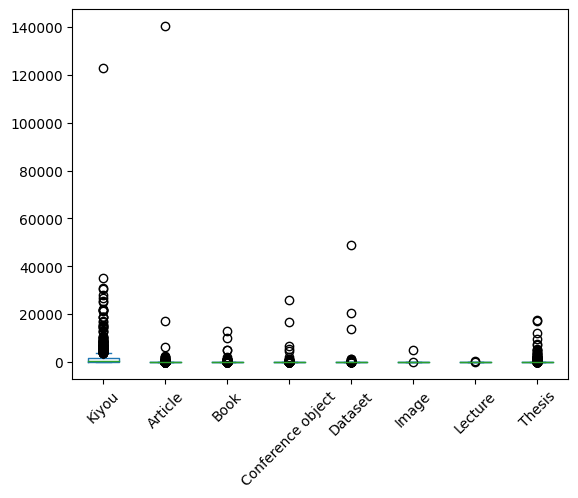
\includegraphics[width=8cm]{./picture/df2205alldstdboxplot.png}
	\caption{外れ値を除いた箱ひげ図}
	\ecaption{Single column figure with caption\\
		explicitly broken by $\backslash\backslash$.}
	\label{fig:box1}
\end{figure}

箱ひげ図は、データのばらつきをわかりやすく表現するための統計図であり、
一番上の線が最大値、一番下の線が最小値、中央の線が中央値などを示し、
丸は外れ値であり値に含まれない。
しかし、図 \ref{fig:box1}では、外れ値ばかりで、このままではばらつきなどが分からない。
そこで、それぞれ大きく外れているデータを以下で確認する。

\begin{lstlisting}[language=Python,breaklines]
	df2205_all_dstd[df2205_all_dstd['Kiyou']>40000]
	df2205_all_dstd[df2205_all_dstd['Article']>40000]
	df2205_all_dstd[df2205_all_dstd['Dataset']>40000]
\end{lstlisting}

結果は
表 \ref{table:outlier1}
のとおりとなった。

'Kiyou'は京都大学が、'Article'は東京工業大学が、'Dataset'は千葉大学が、
それぞれ大きく突出していることが分かる。
ここではデータの全体の感じをつかむため、この3機関を外し、さらにデータの多い'Kiyou'を外して
箱ひげ図を再度作成する。

図 \ref{fig:box2} のとおり、これでもあまり意味のある図にはならなかった。

\begin{figure}[h]
	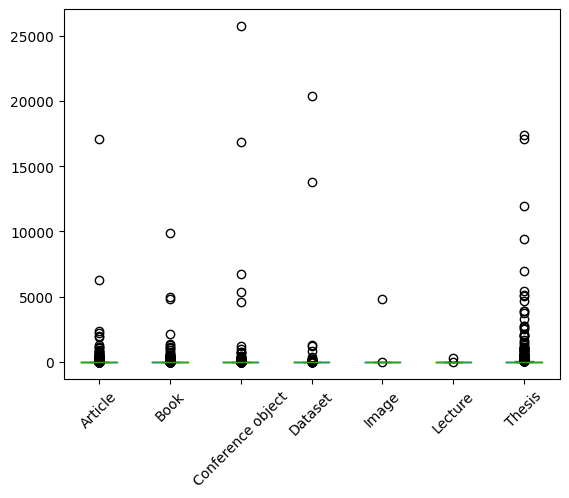
\includegraphics[width=8cm]{./picture/box2.png}
	\caption{外れ値を除いた箱ひげ図}
	\ecaption{Single column figure with caption\\
		explicitly broken by $\backslash\backslash$.}
	\label{fig:box2}
\end{figure}

%3.2
\subsection{特徴量の確認}

相関行列や散布図を用いて特徴量の分布などを確認する。

\begin{figure}[h]
	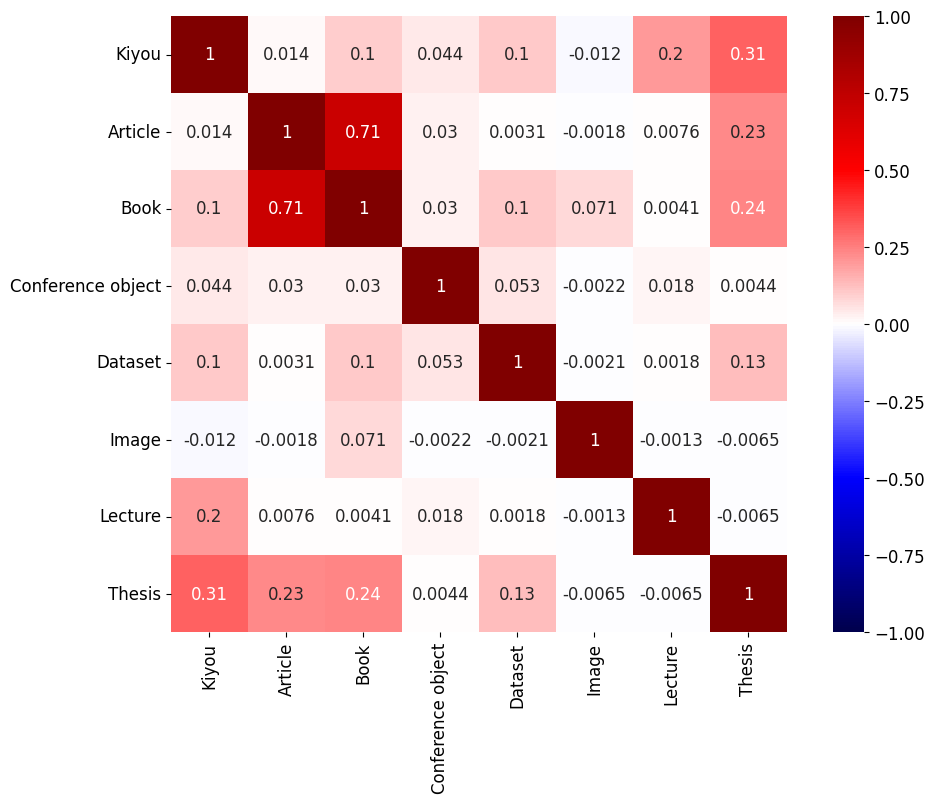
\includegraphics[width=8cm]{./picture/heatmap.png}
	\caption{相関行列のヒートマップ (相関係数の値あり)}
	\ecaption{Single column figure with caption\\
		explicitly broken by $\backslash\backslash$.}
	\label{fig:heatmap12}
\end{figure}

KiyouとArticleはあまり関係がなく、Kiyouと関係があるのはThesisであることが分かる。
これは、日本の機関リポジトリの一般的な印象とも合致する。

%3.3
\subsection{特徴量の標準化}

IRDBのデータから機関リポジトリの特徴を見るためには、量的な特徴を見るのが分かりやすいが、
機関リポジトリごとのコンテンツの量に差がありすぎるため、量以外の特徴がつかみにくい。
ここでは、分析の前処理として、特徴量を標準化する。
標準化はスケーリング(Feature Scaling)の一種で、特徴量間のスケールを変換することである。
特徴量間で異なるスケールを揃えるため、資源タイプごとに、元のデータの平均を0、
標準偏差が1となるように変換する。

\begin{lstlisting}[language=Python,breaklines]
	# 変数の標準化
	df2205_all_std = df2205_all_dstd.apply(lambda x: (x-x.mean())/x.std(), axis=0)
	# 結果を少数以下2桁で丸めて表示
	df2205_all_std.describe().round(2)
\end{lstlisting}

結果は \ref{table:std1} のとおり、
平均が0、標準偏差が1となるように変換されていることが分かる。

%3.3
\subsection{主成分分析}

\begin{lstlisting}[language=Python,breaklines]
	# ライブラリのインポート
	import numpy as np
	import pandas as pd
	import matplotlib.pyplot as plt
	from sklearn.decomposition import PCA
	# 主成分分析の実行
	pca = PCA()
	pca.fit(df2205_all_std)

	# データを主成分に変換
	pca_row = pca.transform(df2205_all_std)

	# 主成分得点
pd.DataFrame(pca_row, columns=["PC{}".format(x + 1)
              for x in range(len(df2205_all_std.columns))]).describe().round(2)
\end{lstlisting}

\onecolumn

% 2段ぶちぬきで下方に図を表示する
\begin{figure}[tb]
	\label{fig:box100000000000000000000000000000}
	% \figref{fig:box1}
	\twocolfig{
		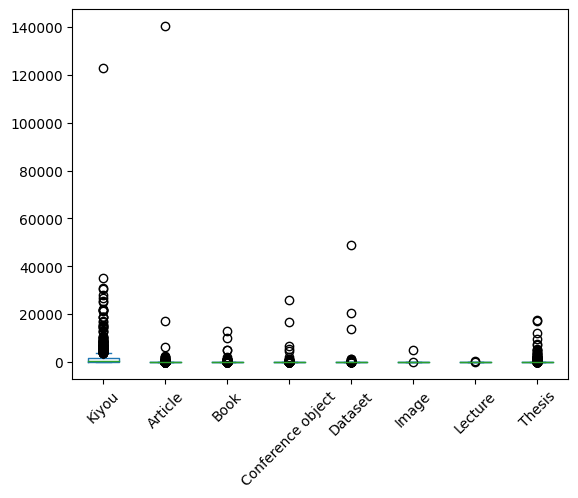
\includegraphics[width=12cm]{./picture/df2205alldstdboxplot.png}
	}
	\twocolcaption{df2205\_all\_dstdの箱ひげ図
	<大き目な図これ[b]だとボトムに図が表示される>}
\end{figure}

%--------------
\begin{table}[tb]
	\caption{df2205\_all\_d.describe\(\)}
	\ecaption{df2205\_all\_d.describe\(\)}
	\label{table:alld}
	\hbox to\hsize{
		\begin{tabular}{p{0.7cm}p{0.7cm}|p{0.7cm}|p{1cm}|p{1cm}|p{1cm}|p{1cm}|p{1cm}|p{1cm}|p{1cm}|p{1cm}|p{1cm}|p{1cm}|p{1cm}}
		% \begin{tabular}{lrrrrrrrrrrrrr}

			&    Kiyou &  Article &    Book &  Cartographic Material &  Conference \par object &  Dataset &  Image &  Lecture &  Patent &  Report &  Sound &  Thesis &  Multiple \\\hline

			count &    792.0 &    792.0 &   792.0 &                  792.0 &              792.0 &    792.0 &  792.0 &    792.0 &   792.0 &   792.0 &  792.0 &   792.0 &     792.0 \\
			mean  &   2011.5 &    249.6 &    78.3 &                    0.0 &               93.8 &    112.7 &    6.1 &      0.4 &     0.0 &     0.0 &    0.0 &   217.2 &       0.0 \\
			std   &   5952.6 &   5051.3 &   643.6 &                    0.4 &             1151.1 &   1948.2 &  170.3 &     10.4 &     0.0 &     0.0 &    0.2 &  1201.0 &       0.0 \\
			min   &      0.0 &      0.0 &     0.0 &                    0.0 &                0.0 &      0.0 &    0.0 &      0.0 &     0.0 &     0.0 &    0.0 &     0.0 &       0.0 \\
			25\%   &    128.0 &      0.0 &     0.0 &                    0.0 &                0.0 &      0.0 &    0.0 &      0.0 &     0.0 &     0.0 &    0.0 &     0.0 &       0.0 \\
			50\%   &    482.5 &      0.0 &     0.0 &                    0.0 &                0.0 &      0.0 &    0.0 &      0.0 &     0.0 &     0.0 &    0.0 &     0.0 &       0.0 \\
			75\%   &   1517.0 &      0.0 &     2.0 &                    0.0 &                0.0 &      0.0 &    0.0 &      0.0 &     0.0 &     0.0 &    0.0 &    19.0 &       0.0 \\
			max   & 123440.0 & 140940.0 & 12907.0 &                   10.0 &            25743.0 &  48965.0 & 4792.0 &    294.0 &     0.0 &     0.0 &    7.0 & 17369.0 &       0.0 \\
			\end{tabular}
	}
\end{table}
%--------------


\begin{table}[tb]
	\caption{df2205\_all\_dstd.describe\(\)}
	\ecaption{df2205\_all\_dstd.describe\(\)}
	\label{table:dstd}
	\hbox to\hsize{\hfil
		\begin{tabular}{l|llllllll}\hline\hline
			      & 1Kiyou        & 2Article      & 2Book        & 5Conference object & 5Dataset     & 6Image      & 7Lecture   & 8Thesis      \\\hline
			count & 789.000000    & 789.000000    & 789.000000   & 789.000000         & 789.000000   & 789.000000  & 789.000000 & 789.000000   \\
			mean  & 1993.239544   & 249.602028    & 78.128010    & 93.576679          & 112.820025   & 6.076046    & 0.372624   & 218.742712   \\
			std   & 5919.979304   & 5044.485846   & 644.070755   & 1152.428752        & 1949.766679  & 170.599642  & 10.431092  & 1200.556001  \\
			min   & 0.000000      & 0.000000      & 0.000000     & 0.000000           & 0.000000     & 0.000000    & 0.000000   & 0.000000     \\
			25\%  & 129.000000    & 0.000000      & 0.000000     & 0.000000           & 0.000000     & 0.000000    & 0.000000   & 0.000000     \\
			50\%  & 487.000000    & 0.000000      & 0.000000     & 0.000000           & 0.000000     & 0.000000    & 0.000000   & 0.000000     \\
			75\%  & 1506.000000   & 0.000000      & 2.000000     & 0.000000           & 0.000000     & 0.000000    & 0.000000   & 20.000000    \\
			max   & 122935.000000 & 140481.000000 & 12883.000000 & 25743.000000       & 48965.000000 & 4792.000000 & 293.000000 & 17369.000000 \\\hline
		\end{tabular}\hfil}
\end{table}


\begin{table}[tb]
	\caption{df2205\_all\_dstd.describe\(\)}
	\ecaption{df2205\_all\_dstd.describe\(\)}
	\label{table:outlier1}
	\hbox to\hsize{\hfil
		\begin{tabular}{l|llllllll}\hline\hline
			                & 1Kiyou & 2Article & 2Book & 5Conference object & 5Dataset & 6Image & 7Lecture & 8Thesis \\\hline
			京都大学'Kiyou'     & 122935 & 1460     & 940   & 1147               & 254      & 0      & 0        & 0       \\
			東京工業大学'Article' & 828    & 140481   & 12883 & 0                  & 11       & 0      & 0        & 7572    \\
			千葉大学'Dataset'   & 10557  & 91       & 134   & 2065               & 48965    & 0      & 0        & 1970    \\\hline
		\end{tabular}\hfil}
\end{table}

\begin{table}[tb]
	\caption{df2205\_all\_dstd.describe\(\)}
	\ecaption{df2205\_all\_dstd.describe\(\)}
	\label{table:std1}
	\hbox to\hsize{\hfil
		\begin{tabular}{l|llllllll}\hline\hline
			      & 1Kiyou & 2Article & 2Book  & 5Conference object & 5Dataset & 6Image & 7Lecture & 8Thesis \\\hline
			count & 789.00 & 789.00   & 789.00 & 789.00             & 789.00   & 789.00 & 789.00   & 789.00  \\
			mean  & -0.00  & -0.00    & 0.00   & 0.00               & 0.00     & 0.00   & -0.00    & 0.00    \\
			std   & 1.00   & 1.00     & 1.00   & 1.00               & 1.00     & 1.00   & 1.00     & 1.00    \\
			min   & -0.34  & -0.05    & -0.12  & -0.08              & -0.06    & -0.04  & -0.04    & -0.18   \\
			25\%  & -0.31  & -0.05    & -0.12  & -0.08              & -0.06    & -0.04  & -0.04    & -0.18   \\
			50\%  & -0.25  & -0.05    & -0.12  & -0.08              & -0.06    & -0.04  & -0.04    & -0.18   \\
			75\%  & -0.08  & -0.05    & -0.12  & -0.08              & -0.06    & -0.04  & -0.04    & -0.17   \\
			max   & 20.43  & 27.80    & 19.88  & 22.26              & 25.06    & 28.05  & 28.05    & 14.29   \\\hline
		\end{tabular}\hfil}
\end{table}

\twocolumn


%====================


\begin{figure}[tb]
	\setbox0\vbox{
		\hbox{\|\begin{figure}[tb]|}
				\hbox{\quad \|<|図本体の指定\|>|}
				\hbox{\|\caption{<|和文見出し\|>}|}
				\hbox{\|\ecaption{<|英文見出し\|>}|}
				\hbox{\|\label{| $\ldots$ \|}|}
				\hbox{\|\end{figure}|}
	}
	\centerline{\fbox{\box0}}
	\caption{1段幅の図}
	\ecaption{Single column figure with caption\\
		explicitly broken by $\backslash\backslash$.}
	\label{fig:single}
\end{figure}


%6
\section{おわりに}

本稿では,



\begin{acknowledgment}
	深謝する.
\end{acknowledgment}

\begin{thebibliography}{2}
\end{thebibliography}
\end{document}

%^^^^^^^^^^^^^^^^^^^
%\subsection{図}
%1段の幅におさまる図は,
%\figref{fig:single} の形式で指定する.
%位置の指定に \|h| は使わない.
%また,図の下に和文と英文の双方の見出しを,
%\|\caption| と \|\ecaption| で指定する
%図の参照は \|\figref{<|ラベル\|>}| を用いて行なう.

%また紙面スペースの節約のために,
%1つの \|figure|(または \|table|)環境の中に複数の図表を並べて表示したい場合には,
%\figref{fig:left} と \tabref{tab:right} のように個々の
%%図表と各々の \|\caption|/\|\ecaption| を \|minipage| 環境に入れることで実現できる.
%なお図と表が混在する場合,
%\|minipage| 環境の中で\|\CaptionType{figure}| あるいは \|\CaptionType| \|{table}| を指定すれば,
%外側の環境が \|figure| であっても \|table| であっても指定された見出しが得られる.


%4.7.1
%\subsubsection{参考文献の参照}
%本文中で参考文献を参照する場合には\|\cite|を使用する.
%参照されたラベルは自動的にソートされ,\|[]|でそれぞれ区切られる.
%
%\begin{quote}
%	文献 \|\cite{companion,okumura}| は \LaTeX の総合的な解説書である.
%\end{quote}
%文献リストはBiB\TeX と\verb+ipsjunsrt.bst+(参照順)
%または\verb+ipsjsort.bst+(アルファベット順)を用いて作り,
%\verb+\bibliograhpystyle+と\verb+\bibliography+コマンドにより
%また製版用のファイル群には\verb+.bib+ファイルではなく\verb+.bbl+ファイルを必ず含めることに
